\section{Introduccion}
Para este trabajo intentaremos resolver la planificacion de caminos de un robot movil utlizando la tecnica de Rapidly-exploring random tree. Para ello implementaremos el algoritmo y luego realizaremos diferentes experimentaciones sobre el mismo con la intención de ver como se comporta.

A continuación respondemos las preguntas requeridas en el informe.
\\
\\
\textit{Explicar como definieron el ”area cercana al goal”. ¿Tomaron en cuenta elangulo $\theta$? ¿Como?.}


Para definir el area mas cercana al goal definimos un rectangulo con constantes GOAL\_AREA\_X, GOAL\_AREA\_Y con centro en el goal.  Para considerar el angulo de las poses aleatorias que generamos, en caso de caer en el area definida anteriormente cercana al goal dicho angulo es aleatorio en un rango ($\-pi/2\theta_{goal}$, $\pi/2 \theta_{goal}$).

Las demas configuraciones, fuera del area definida, son completamente aleatorias.
\\
\\
\textit{Explicar que definicicon de distancia utilizaron. ¿Como integran el angulo $\theta$?.}
\\Para definir la distancia utilizamos una formula que pondera la distancia euclidea y la diferencia de orientaciones entre las dos poses.

Para definirlo mas precisamente, dadas dos configuraciones $c_1$ y $c_2$ la función de distancia estará dada por:

$$K_{dist}. distancia\_euclidea(C_1,C_2) + K_{Ori}. dist_{Ori}(C_1,C_2) $$

Donde $K_{dist}$, $K_{Ori}$ son los pesos de importancia que le daremos a cada una de estas metricas. $distancia\_euclidea(C_1,C_2)$ es la norma 2 entre el x,y de cada configuración y $dist_{Ori}(C_1,C_2)$ es el modulo de la distancia angular entre el $\theta$ de $c_1$ y $c_2$ 
\\
\\
\textit{Explicar como establecieron ”discretizaron” el espacio de posibilidades a partir de la ”configuracion mas cercana”.}

Se cuenta con dos variables que nos permiten ajustar el stepping en velocidad lineal (wx\_step) y angular (wz\_step).

A partir de la configuracion mas cercana tomaremos un numero discreto de acciones posibles, dejando constante wx\_step y variando la direccion en cero menos uno o uno wz\_step.

De todas las discretizaciones posibles nos quedamos con aquella mas cercana al $q_{new}$
\\
\\
\textit{Explicar como resolvieron esta comprobacion.}

Para resolver la comprovacion de colisión, definimos un area rectangular alrededor de la nueva configuracion verificando si una cantidad de puntos de ese rectangulo estan o no libres. En caso de encontrarse todos libres decimos que no se producen colisiones en caso contrario diremos que hay colisiones y ese punto no será valido.

\section{Experimentación}

En esta sección veremos como afectan las variaciones en el stepping de velocidad y el goal bias al algoritmo y sacaremos las concluciones convenientes.

Para toda esta sección se utilizaran los valores

\begin{itemize}
\item $GOAL\_AREA\_X$ 1
\item $GOAL\_AREA\_Y$ 1
\item $K\_DIST$ 0.8
\item $K\_ORI$ 0.2
\end{itemize}

Como primera instancia variaremos el stepping de velocidad dejando constante el goal bias en $0.6$.

Variando el stepping en la velocidad lineal a $0.005$ y varianndo el de la velocidad angular a $0.002$ obtenemos el siguiente grafico:



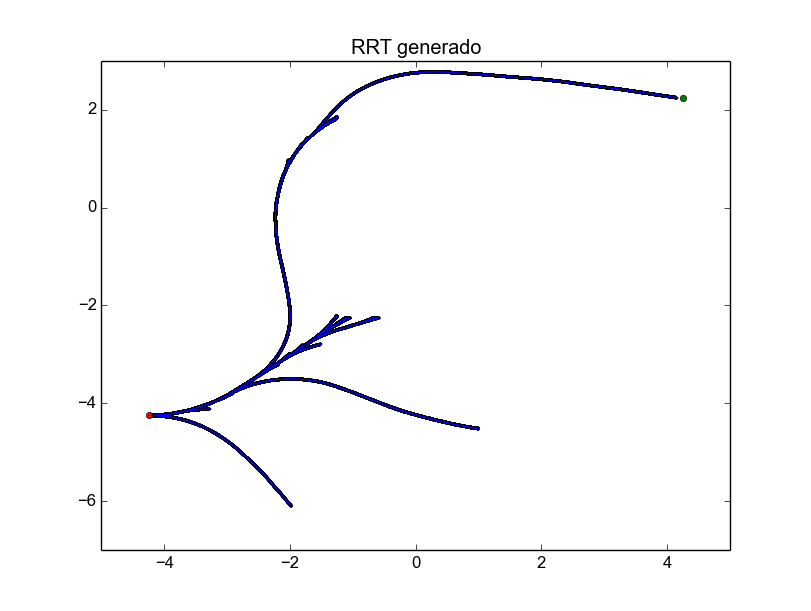
\includegraphics[scale=0.5]{velocidad/stepping_Bajo1.png}
%stepping_Bajo1.png

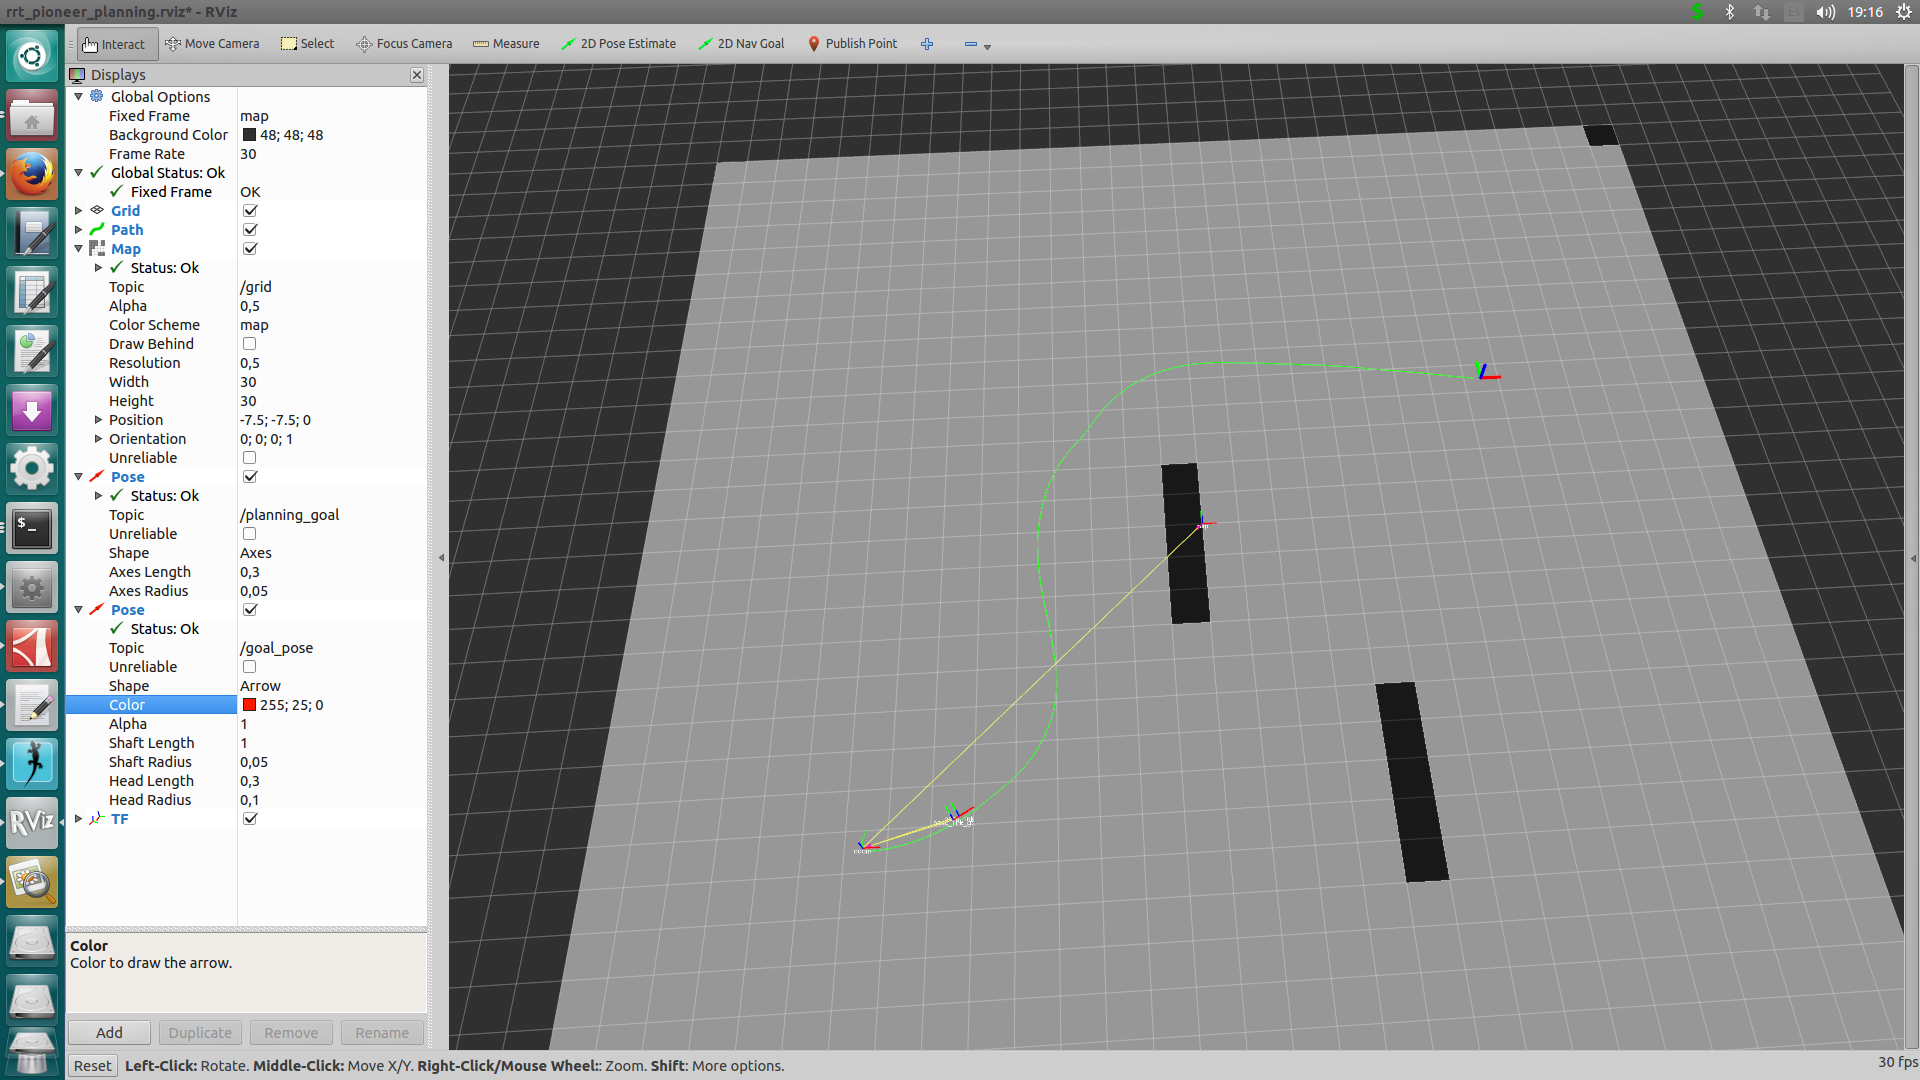
\includegraphics[scale=0.3]{velocidad/stepping_Bajo_rviz1.png}
%stepping_bajo_rviz1.png

Si bien llega al objetivo fueron necesarias muchas mas iteraciones de las que venian por default. Con $20000$ iteraciones el arbol no lograba llegar a destino.

Como segunda prueba aumentamos el stepping a 0.5 y 0.3 respectivamente. El grafico resultante es el siguiente:

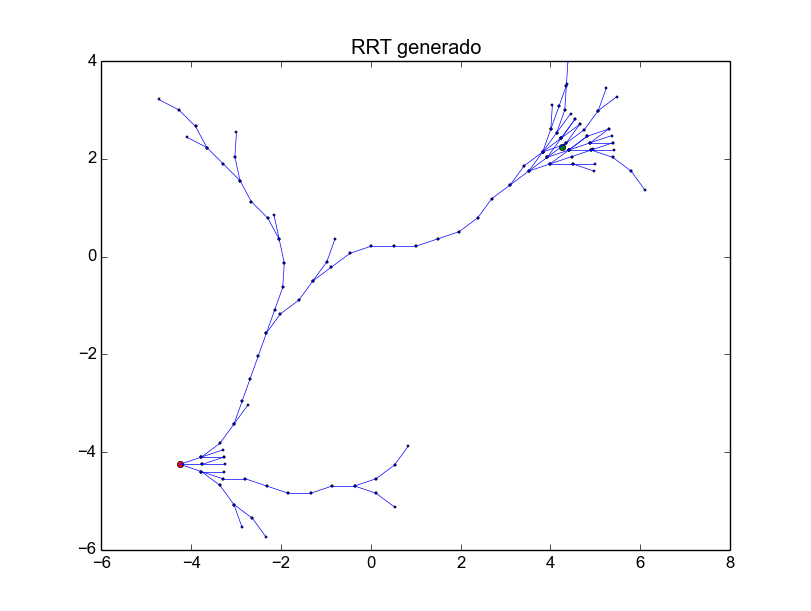
\includegraphics[scale=0.5]{velocidad/stepping_alto1.png}
%stepping_alto1.png

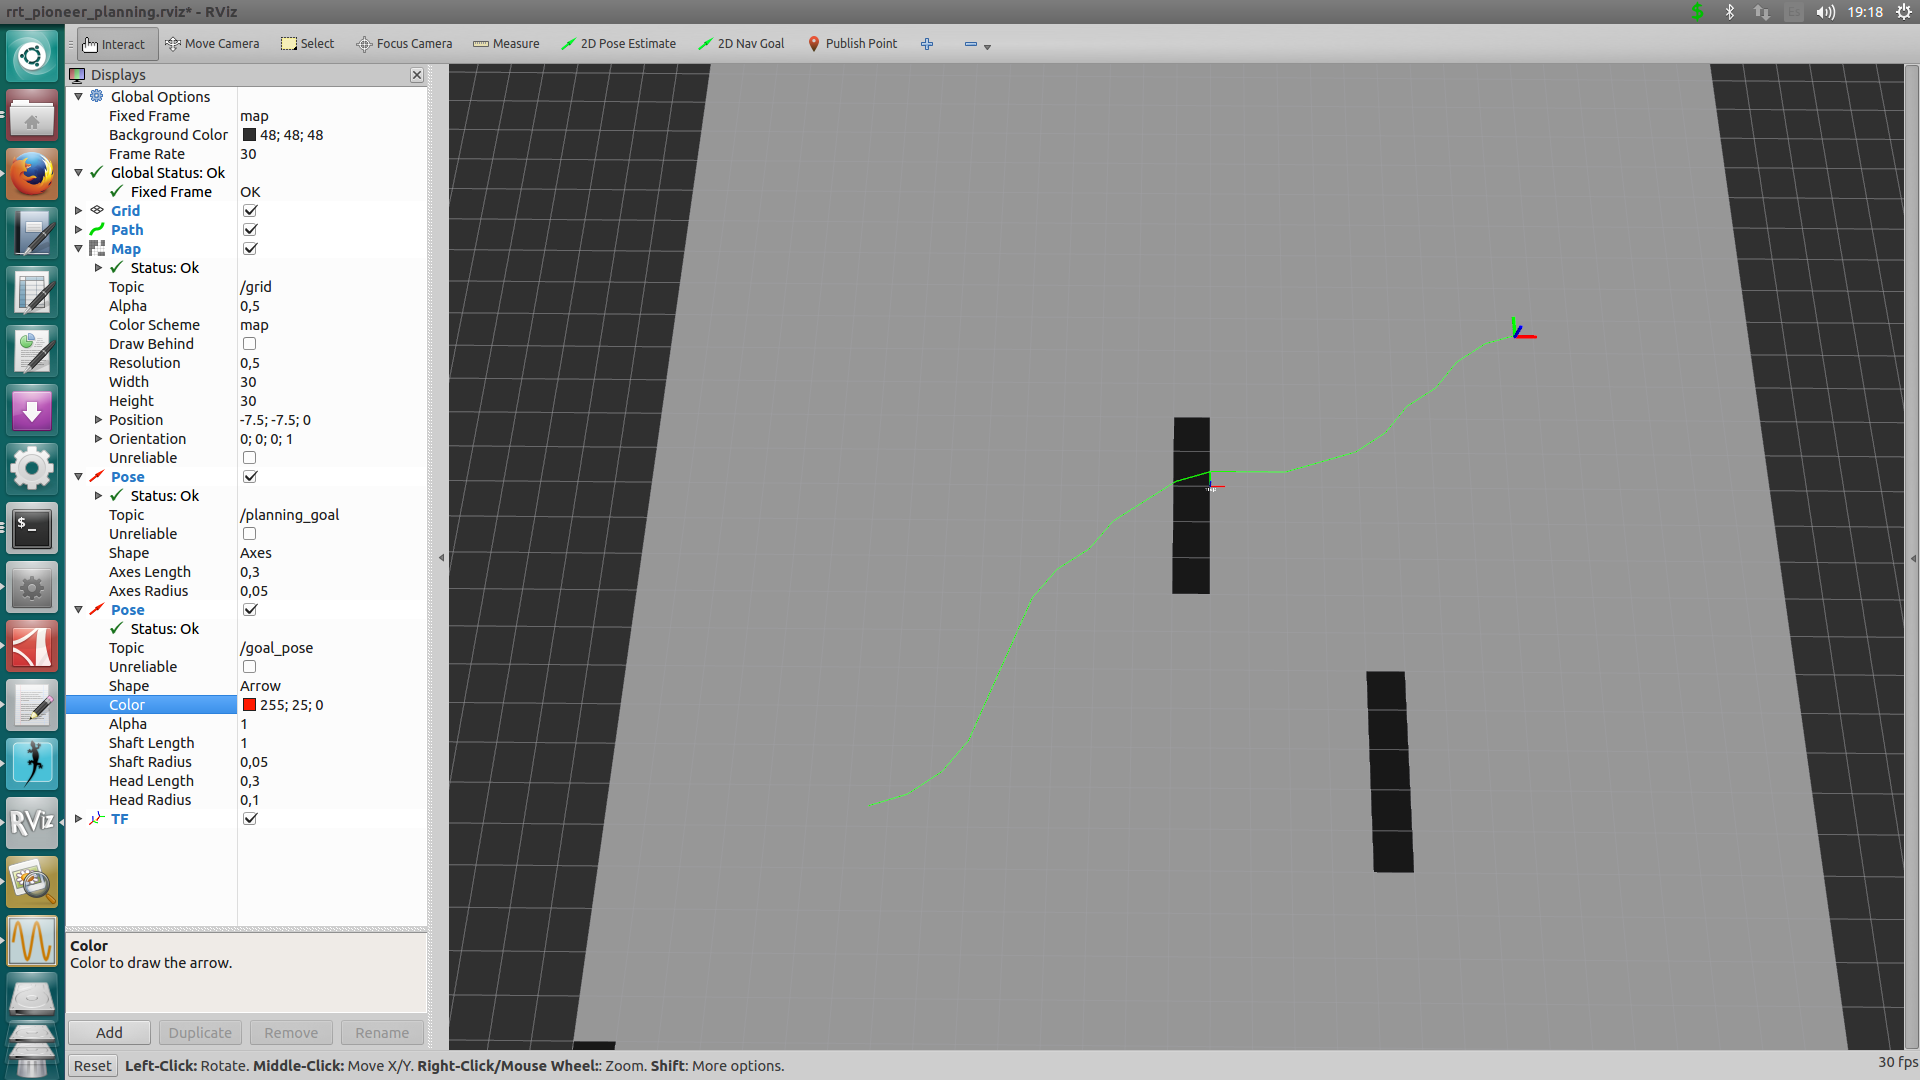
\includegraphics[scale=0.3]{velocidad/stepping_alto_rviz1.png}
%stepping_alto_rviz1.png

Si bien el algoritmo llego a destino, este camino no es valido, ya que como como podemos ver en rviz pasa por entre medio de un obstaculo. Creemos que esto se debio a que la baja granularidad empeoró el calculo de las posiciones intermedias libres.

Realizamos la misma experimentación para la segunda escena provista por la catedra. Para el stepping bajo observamos el siguiente grafico:

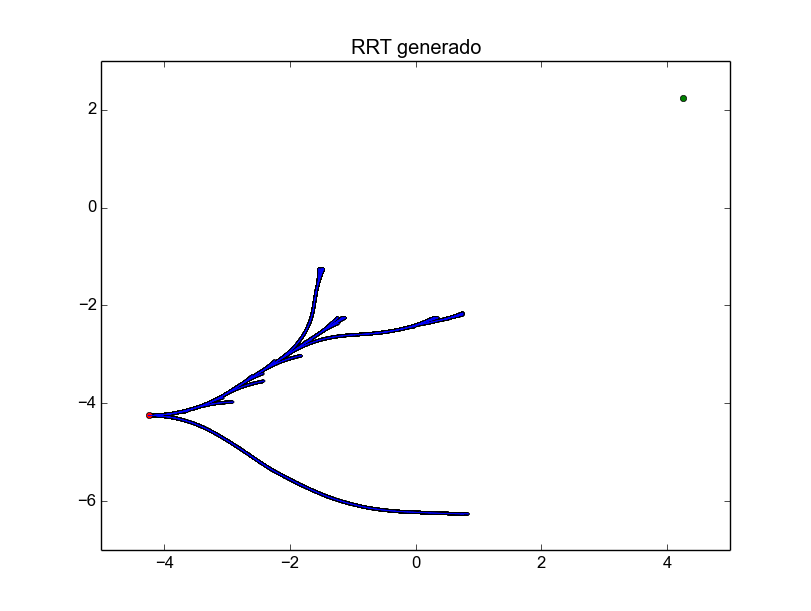
\includegraphics[scale=0.5]{velocidad/stepping_bajo2.png}
%stepping_bajo2.png

Esto se debio a que posiblemente el pequeño stepping tanto en velocidad angular como en velocidad lineal no le permitio llegar al goal en las iteraciones provistas.

Para el stepping alto:

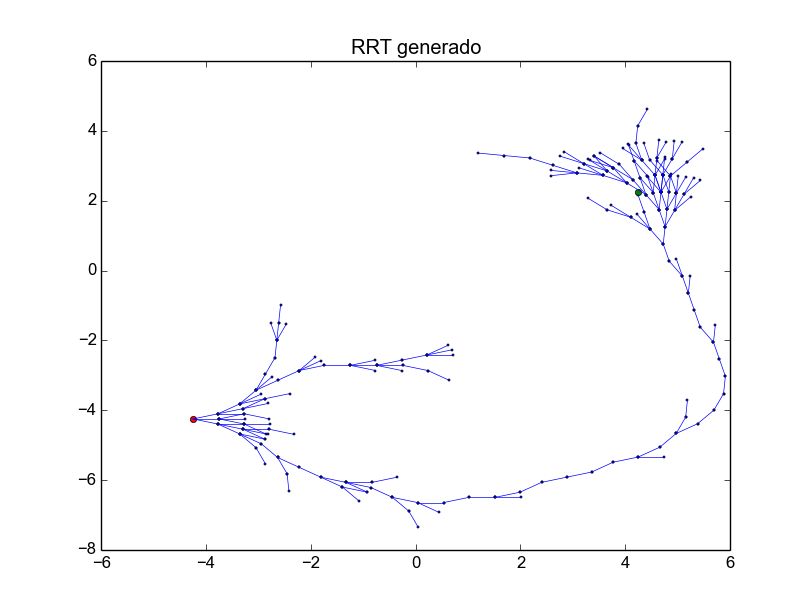
\includegraphics[scale=0.5]{velocidad/stepping_alto2.png}
%stepping_alto2.png

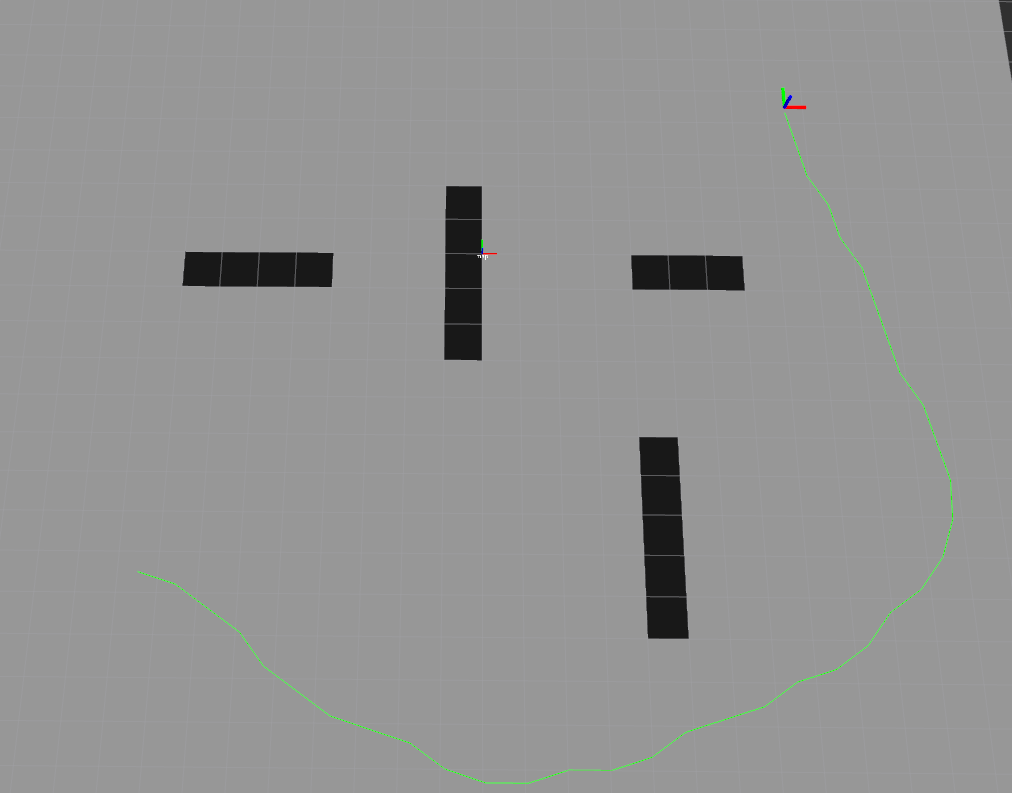
\includegraphics[scale=0.3]{velocidad/stepping_alto_rviz2.png}
%stepping_alto_rviz2.png

Es posible llegar a la solución sin embargo es posible observar al acercarse a la posicion del goal no le dio en angulo para correcto y tuvo que continuar con una exploración poco acertada.
%
%
%
En cuanto a la experimentación sobre el goal bias llegamos a la conclusión de que valores muy altos y muy bajos hacen que no siempre se logre conseguir una trayectoria válida hacia destino.

Comenzamos mostrando un escenario con goal bias \textit{alto} de $0.8$, recordemos que esto nos dice que el $80\%$ de las configuraciones aleatorias van a caer en el area \textit{cercana} al goal que definimos.

En la escena: rrt\_pioneer\_planning el árbol resultante fue el siguiente:

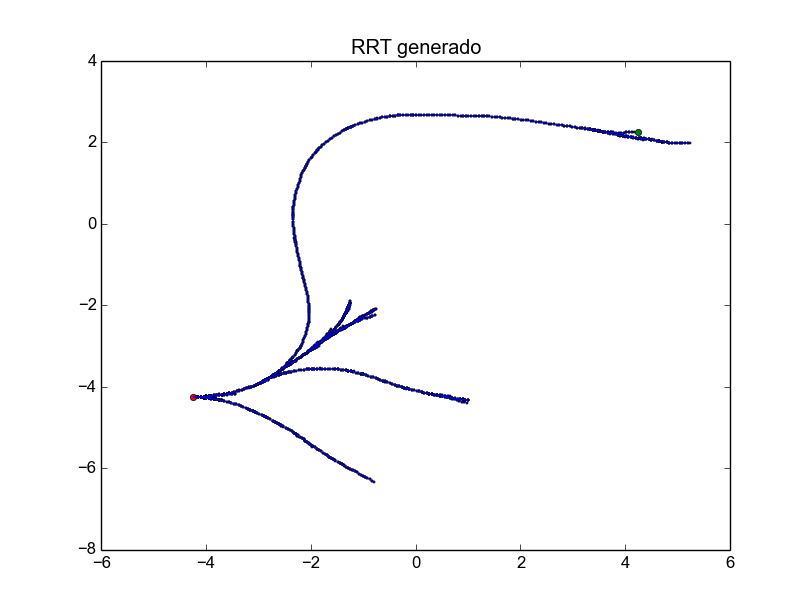
\includegraphics[scale=0.5]{tp4_imagenes/informe_goal_bias_08.png}
%%informe_goal_bias_08

Si bien consideró un par de caminos que no lo llevaba al goal, la trayectoria es bastante directa y no se obtuvo un arbol muy ramificado. La elección del goal bias puede considerarse acertada para este escenario.

%%informe_goal_bias_08_rviz x3
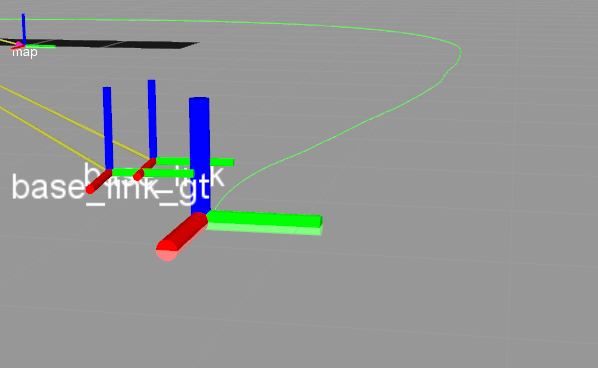
\includegraphics[scale=0.5]{tp4_imagenes/informe_goal_bias_08_rviz1.png}


Podemos ver en rviz que las poses finales son bastante cercanas a la del goal

A medida que disminuimos este valor el arbol comienza a randomizarse, como caso extremo mostramos lo que sucede con $goal\_bias$ $0.1$, el arbol que se obtiene es este:

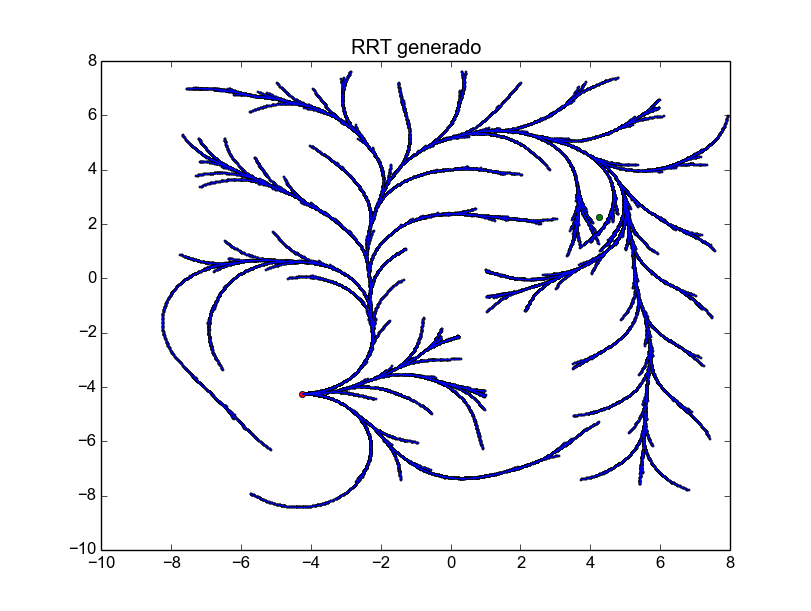
\includegraphics[scale=0.5]{tp4_imagenes/informe_goal_bias_01.png}
%%informe_goal_bias_01

La gran diferencia de este caso con el anterior es el nivel de exploración sobre el mapa. Al tener casi todos los puntos aleatorizados en cualquier posición (cercana o lejana al goal), los posibles caminos no están lo suficientemente sesgados para que se dirija al goal. Si bien algunos de los subcaminos se acercan nunca es lo suficiente a una pose (con enfasis en la orientación) parecida a la del destino.


Para otros escenarios el comportamiento no es necesariamente similar, ya vimos que un goal\_bias bajo no nos daba buenos resultados, pero si mantenemos el $0.8$ anterior ya no encuentra el trayecto

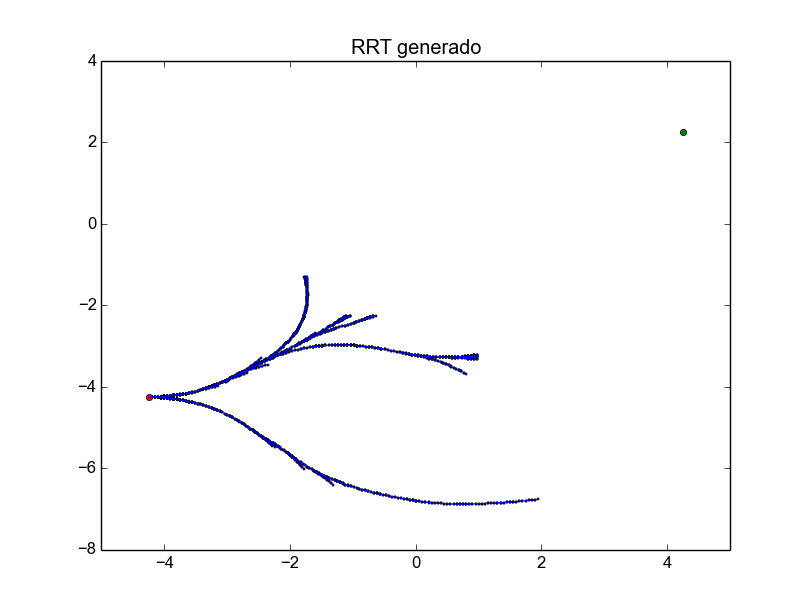
\includegraphics[scale=0.5]{tp4_imagenes/informe_goal_bias_dificil_08.png}
%%informe_goal_bias_08_dificil

Lo que está pasando en este caso es que al tener muchos más obstáculos y tan pocos puntos aleatorios fuera del área cercana al goal es mucho mas costoso formar caminos que se alejen de los objetos que causan las colisiones. 

Vale la pena destacar que agregando más iteraciones al algoritmo esto  puede solucionarse (de todas formas no es la solución optima al problema).

Para mejorar esto es conveniente no usar un goal tan cercano a 1, bajandolo a 0.6 logra mitigarse el problema anterior y se llega a destino.

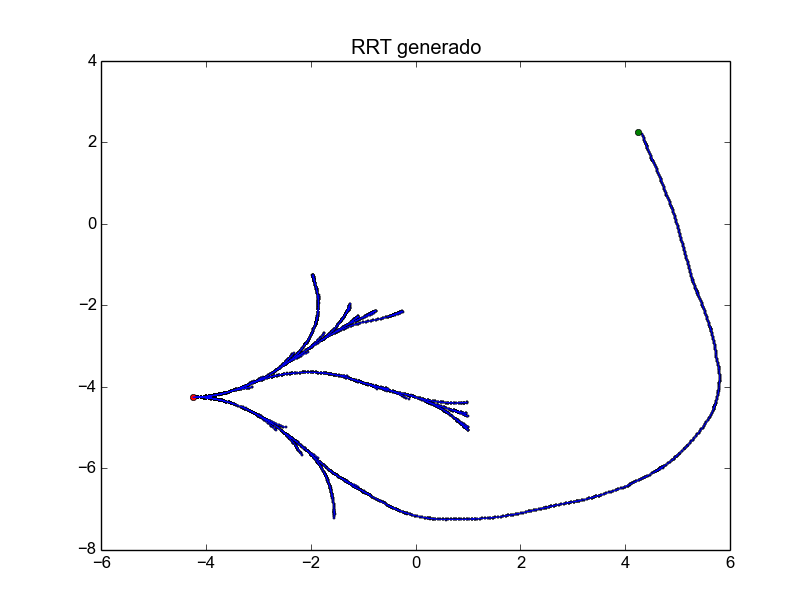
\includegraphics[scale=0.5]{tp4_imagenes/informe_goal_bias_dificil_06.png}
%%informe_goal_bias_06_dificil

Los resultados son claros ya que hay poca diferencia entre los caminos que considera respecto al caso anterior, pero al elegir más configuraciones mejor distribuidas en el mapa sale de las zonas de colisiones y finalmente logra dirigirse al goal.

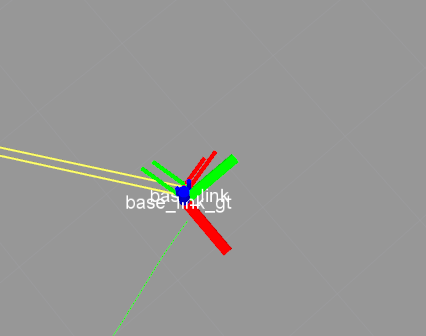
\includegraphics[scale=0.5]{tp4_imagenes/informe_goal_bias_dificil_06_rviz1.png}
%%informe_goal_bias_06_dificil_rviz x3

La pose final que encuentra no fue tan buena como en el escenario anterior pero sigue siendo una buena aproximación al goal.

Si bien no aporta mucho más a lo discutido anteriormente vale la pena mencionar que el caso con bias muy bajo tampoco es bueno en este escenario

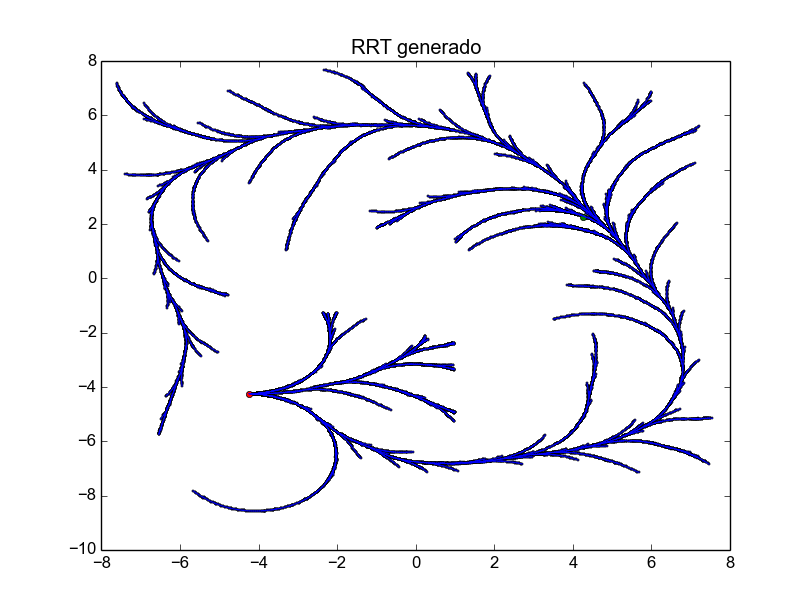
\includegraphics[scale=0.5]{tp4_imagenes/informe_goal_bias_dificl_01.png}
%%informe_goal_bias_01_dificil

En esta ocasión se acerco al goal pero ninguno de los caminos le permitió obtener una orientación cercana.


% Para cada una de las escenas de vrep provistas plantear (configurando el archivo launch):
% • Dos ejecuciones, uno con goal bias ”bajo” y uno ”alto”.
% • Dos conjuntos de valores para el stepping de velocidades. Uno con ”ve-
% locidades muy demandantes” y uno con ”velocidades poco demandantes”.
% Presentar un gr ́
% afico con el  ́arbol generado por el algoritmo RRT en cada
% situaci ́
% on. ¿En que casos se pudo encontrar soluci ́on?, ¿Como resulto el seguimiento
% de la trayectoria a lazo abierto?. En los casos en que se pudo encontrar un
% camino, presentar una captura de pantalla con la posici ́on final del pioneer en
% el RViz
% ¿Como se podr ́ıa mejorar el algoritmo RRT de manera de ”gu ́ıarlo” de manera
% m ́
% as eficiente hacia el goal?. Contemplar el algoritmo A*.